\section{Ejercicio 3: Escapando}

  \begin{figure}[H]
    \begin{center}
      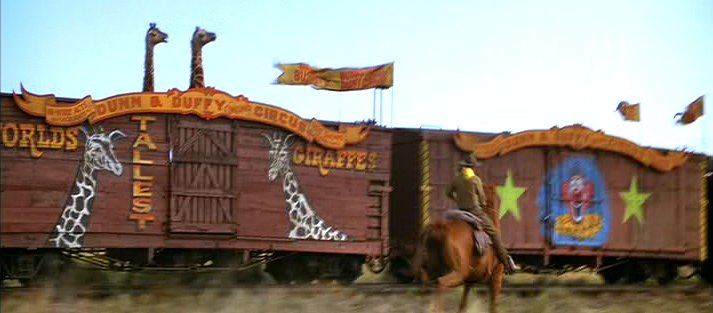
\includegraphics[width=0.4\columnwidth]{imagenes/tren.jpg}
      \caption{El tren se va}
    \end{center}
  \end{figure}


    % 1. Describir detalladamente el problema a resolver dando ejemplos del mismo y sus soluciones.
    \subsection{Descripción del problema}

        \par Luego de colectar todas las piezas Indy se encuentra conforme con lo obtenido, aunque todavía no comprende lo que dice, el material encontrado lo ayudará a conseguir subsidios para continuar con la investigación.
        \par Ya se encuentran en el lugar donde estaba la cruz en el mapa, hay unos carritos sobre vias que parecen dirigirse hacia afuera de la fortaleza. De repente se escuchan unos ruidos muy fuertes desde adentro del laberinto. Luego de romper todas las paredes internas buscando las partes de la tabla se dieron cuenta que se esta desplomando toda la estructura, por lo que deben hacer un escape rápido. \par Al lado del carrito se encuentra un gráfico con la red de las vias. Hay puntos numerados que parecen indicar lugares donde los carritos pueden hacer paradas (estaciones). La estación 1 es donde se encuentran, y la última estación es donde quieren llegar. Las estaciones estan unidas con vías. Al lado de cada vía hay flechas con un número indicando el tiempo que tarda en moverse entre dos estaciones.
        \par Ayudemos a escapar cuanto antes a todos antes de que mueran aplastados.
        \\~\\
        \textbf{En resumen...}
        \par Dado una cantidad de estaciones y una cantidad de vías que cada una conecta un par de estaciones con cierta duración, se debe encontrar la forma más rápida de llegar de la primera a la última estación.
        \\~\\
        \textbf{Formato de entrada:} El formato de entrada contiene dos numeros. La cantidad de estaciones N, y la cantidad de vı́as M. Luego siguen M lı́neas, cada una contiene tres enteros A, B y C que indican que ir de A a B tarda C segundos. Las estaciones estan númeradas de 1 a N.
        
        \begin{verbatim}
        N M
        A_1 B_1 C_1
        ...
        A_M B_M C_M
        \end{verbatim}
        
        \textbf{Formato de salida:} La primera lı́nea deberá tener un entero T indicando el mı́nimo tiempo para ir de la estación 1 a la estación N. Si no es posible, devolver −1. En caso de que sea posible, la segunda lı́nea deberá tener un entero S indicando la cantidad de estaciones que debe recorrer y la tercera lı́nea contendrá S enteros que indican la forma de escapar lo más rápido posible.
        
        \begin{verbatim}
        T
        S
        E_1 E_2 ... E_S
        \end{verbatim}
        
        \textbf{Ejemplos:}
        
        1)
        Una posible entrada válida sería:
        
        \begin{verbatim}
        N = 5   M = 5
        [A B C] = { 1 2 1, 2 3 4, 3 4 5, 4 5 3, 2 4 2 }
        \end{verbatim}

        Y su salida válida sería:

        \begin{verbatim}
        T = 6   S = 4
        E = { 1 2 4 5 }
        \end{verbatim}

        2)
        Otra posible entrada válida sería:
        
        \begin{verbatim}
        N = 6   M = 9
        [A B C] = { 1 2 8, 1 3 4, 2 4 2, 2 5 1, 3 5 1, 4 5 1, 5 4 10, 4 6 1, 5 6 7 }
        \end{verbatim}

        Y su salida válida sería:

        \begin{verbatim}
        T = 11  S = 4
        E = { 1 2 4 6 }
        \end{verbatim}

        3)
        Otra posible entrada válida sería:
        
        \begin{verbatim}
        N = 3   M = 2
        [A B C] = { 1 2 1, 2 1 1 }
        \end{verbatim}

        Y su salida válida sería:

        \begin{verbatim}
        T = -1
        \end{verbatim}


    % 2. Explicar de forma clara, sencilla, estructurada y concisa, las ideas desarrolladas para la resolución del problema. Utilizar pseudocódigo y lenguaje coloquial (no código fuente). Justificar por qué el procedimiento resuelve efectivamente el problema.
    \subsection{Solución propuesta}
    
    \par Como solución decidimos modelar el problema en un grafo y usar el \emph{Algoritmo de Dijkstra} para obtener el camino mínimo de manera tal que no supere la complejidad pedida.

    \par Las estaciones y los recorridos serán modelados en un grafo en el cual los vértices representarán a las estaciones, las aristas representarán a las vías, y el peso de cada arista representará al tiempo que se tarda en llegar de una estación a la otra.
    \par Este grafo será implementado con una lista de adyacencia. Es decir, una lista de N posiciones, siendo N la cantidad de estaciones. Cada posición i tendrá una lista con las estaciones vecinas alcanzables desde la estación i. Cada estación vecina j será una tupla de dos valores: el número de la estación j y el tiempo que se tarda en llegar desde la estación i a la estación j.
    
     \\~\\
     
    \begin{algorithmic}
    \State \Comment {O(m)}
    \Function{Grafo ListAdy}{Int estaciones, Int vias, Lista(estacion1, estacion2, distancia) recorridos}
        \State $listAdy \gets estaciones * \{\}$ \Comment {O(1)}
        \For{$rec \in recorridos$} \Comment {O(m)}
            \State $listAdy_{rec.estacion1}.agregar((rec.estacion2, rec.tiempo))$ \Comment {O(1)}
        \EndFor
        \State \Return {$listAdy$}
    \EndFunction
    \end{algorithmic}
     
     \\~\\
    
    \par Luego se implementará el algoritmo de Dijkstra sobre esta lista de adyacencia. Es decir, siendo N la cantidad de estaciones, el algoritmo resolverá de manera eficiente como llegar de la estación 1 a la N de la forma más rápida.
    \par El algoritmo de Dijkstra recorre los nodos en el orden de distancia al origen. El siguiente nodo a visitar lo elige como el más cercano al origen que no haya sido visitado anteriormente. Y al visitar un nodo actualiza la distancia de sus vecinos y sus respectivos precedentes.
    
     \\~\\
    
    \begin{algorithmic}
    \State \Comment {O((n+m) * $\log n$)}
    \Function{Dijkstra}{Grafo listAdy, Int cantEstaciones}
        \State $time\gets cantEstaciones * \infty$ \Comment {O(n)}
        \State $antecesores\gets cantEstaciones * \infty$ \Comment {O(n)}
        \State $noVisitados\gets ColaDePrioridad((tiempo, estacion))$ \Comment {O($\log n$)}
        \State $time_{0}\gets 0$ \Comment {O(1)}
        \State $noVisitados.encolar((0,0))$ \Comment {O($\log n$)}
        \While {$noVisitados$ tenga elementos} \Comment {O((n+m) * $\log n$)}
            \State $estacion\gets noVisitados.extraerMin()$ \Comment {O($\log n$)}
            \For{$vecino \in listAdy[estacion]$} \Comment {O(m * $\log n$)}
                \If {$time_{vecino} > time_{estacion} + tiempo_{vecino, estacion}$} \Comment {O(1)}
                    \State $nuevoTiempo\gets noVisitados.actualizarPrioridad()$ \Comment {O($\log n$)}
                    \State $time_{vecino}\gets nuevoTiempo$ \Comment {O(1)}
                    \State $antecesores_{vecino}\gets estacion$ \Comment {O(1)}
                \EndIf
            \EndFor
        \EndWhile
        \State \Return {$time_{cantEstaciones}, obtenerSalida(antecesores)$} \Comment {O(n)}
    \EndFunction
    \end{algorithmic}
    
     \\~\\
    
    \par  Para este caso en particular, el algoritmo usará un árbol binario para almacenar los nodos no visitados. De esta manera, se podrá extraer el nodo más cercano al origen y actualizar la prioridad de un nodo cuando se encuentre una distancia menor en complejidad logarítmica.
    \par Para que la función devuelva lo pedido, se obtiene el tiempo mínimo que se tarda en llegar de la estación inicial a la estación final con el valor de la última posición de la lista \emph{time}. Y por otro lado, a partir de la lista \emph{antecesores} se obtiene el recorrido más rápido, con sus estaciones.

    \par El problema planteado se puede visualizar como un contexto en el cual se tiene un grafo con varios vértices (estaciones), con distintas aristas (vías), cada una con su peso (tiempo en llegar de una estación a la otra). Y a partir de este grafo, se desea obtener el camino mínimo desde el primer nodo hasta el último.
    \par Según los algoritmos vistos en la cátedra, la mejor solución para este tipo de problemas es aplicar a ese grafo el \emph{Algoritmo de Dijkstra}, el cual resuelve eficientemente el camino con menos peso para llegar de cierto nodo inicial a cierto nodo final.
    \par Dado este análisis del problema, se llega la conclusión de que el procedimiento desarrollado es una solución eficiente que lo resuelve.
   
    \subsection{Complejidad teórica}
        Dada la explicación anterior, el algoritmo tiene complejidad temporal de $O((N+M) * \log N)$ donde $N$ es la cantidad de estaciones y $M$ es la cantidad de vías.
        Esto se da debido a que se usa el algoritmo de Dijkstra con una lista de prioridad implementada con un árbol binario.
        Notar que $O((N+M) * \log N)$ puede ser peor $O(n^{2})$. Conviene usar min heap o un árbol cuando el grafo es esparso, es decir, cuando M es mucho menor que N^{2}.
    

    % 4. Dar un código fuente claro que implemente la solución propuesta. Se deben incluir las partes relevantes del código como apéndice del informe impreso entregado.

    % 5. Realizar una experimentación computacional para medir la performance del programa implementado. Usar un conjunto de casos de test en función de los parámetros de entrada, con instancias aleatorias e instancias particulares (de peor/mejor caso en tiempo de ejecución, por ejemplo). Presentar en forma gráfica una comparación entre los tiempos medidos y la complejidad teórica calculada y extraer conclusiones.
    \subsection{Experimentación}

        Al igual que con los otros dos ejercicios, se realizaron pruebas experimentales para verificar que el tiempo de ejecución del algoritmo cumpliera con la cota asintótica de $O((N+M) * \log N)$, teóricamente demostrada para el peor caso...
        \par Se plantearon los siguientes casos relevantes para verificar su funcionamiento:
        \par - Se corrieron casos aleatorios alterando la cantidad de vértices, aristas y pesos de cada arista.

        En la siguiente figura, se puede observar los resultados de correr la experimentación explicada. Se muestra el tiempo de procesamiento en función de los vértices...

        \begin{figure}[H]
          \begin{center}
            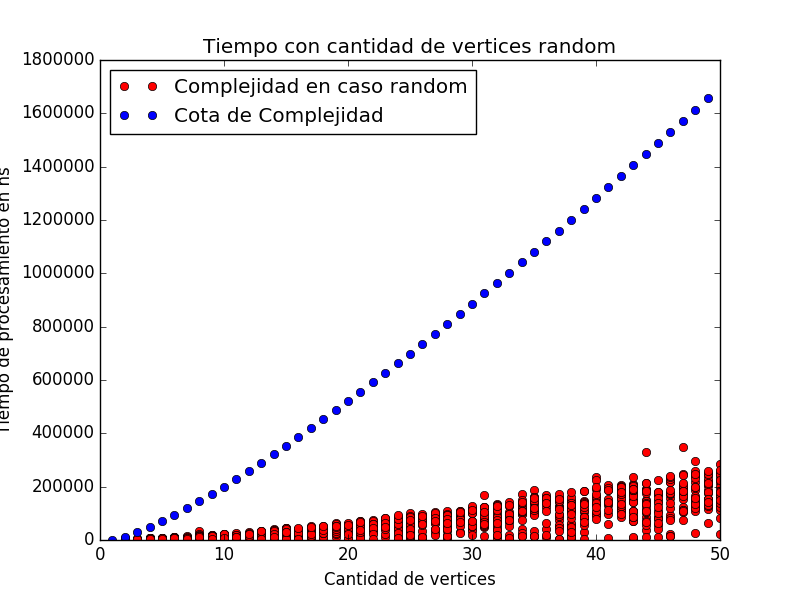
\includegraphics[width=0.7\columnwidth]{../exp/ej3casosRandomVertices.png}
            \caption{}
          \end{center}
        \end{figure}

        En la siguiente figura, se puede observar los resultados de correr la experimentación explicada. Se muestra el tiempo de procesamiento en función de las aristas...

        \begin{figure}[H]
          \begin{center}
            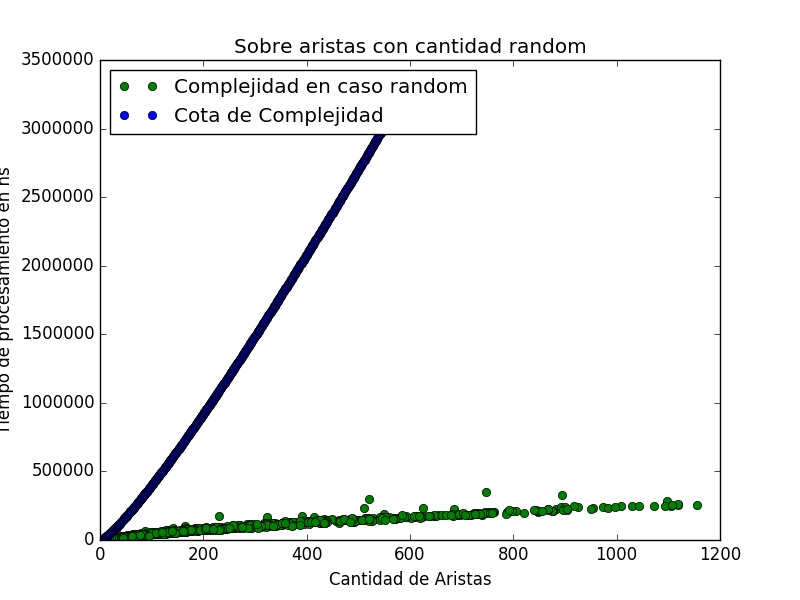
\includegraphics[width=0.7\columnwidth]{../exp/ej3casosRandomAristas.jpeg}
            \caption{}
          \end{center}
        \end{figure}

        Se puede visualizar que los resultados obtenidos en los experimentos con entradas aleatorias difieren mucho con respecto a la cota de complejidad teórica. Esto se debe a que los casos no fueron suficientemente grandes como para alcanzarla. 
        También se puede observar en el gráfico que el tiempo de ejecución no depende únicamente de la cantidad de vértices dado que un grafo puede ser muy denso y esto daría al Algoritmo de Disjktra muchas más posibilidades para recorrer que en el caso en el que hayan pocas aristas. Por eso en el gráfico de tiempo en función de aristas se ven los puntos agrupados en una pendiente creciente, y en el gráfico de tiempo en función de vértices puntos más dispersos.

        \par - Se corrieron casos particulares en los que se debería alcanzar la cota de complejidad. Es decir, los peores casos.
        Para esto, se probó con grafos de n vértices. Para cada vértice i (1 $\leq$ i $<$ n), existe todas las posibles aristas (i, j) tal que j pertenece al intervalo (i, n). Y luego un arista (n-1, n). 
        De esta manera el algoritmo tendrá que recorrer todos los vértices para obtener el camino mínimo.

        \par - Se corrieron casos particulares en los que la complejidad debería ser la mínima posible, es decir, los mejores casos.
        Para esto, se probó con grafos en los que únicamente existía un arista que unía el primer vértice con el último.

        En la siguiente figura, se puede observar los resultados de correr la experimentación explicada...

        \begin{figure}[H]
          \begin{center}
            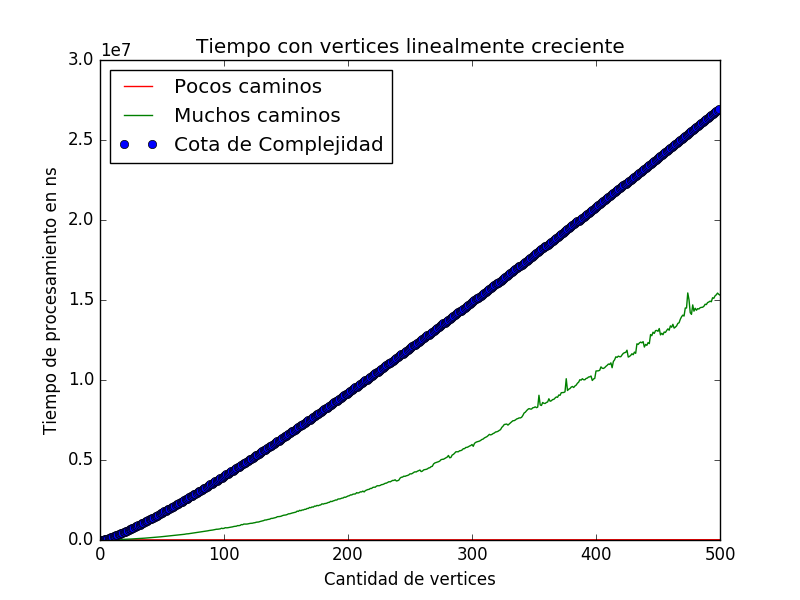
\includegraphics[width=0.7\columnwidth]{../exp/ej3tamanosFijos.png}
            \caption{}
          \end{center}
        \end{figure}

        Se puede visualizar para los peores casos una curva creciente que tiende a la cota de complejidad. Esto se debe a que el Algoritmo de Dijkstra recorre todos los caminos posibles para llegar al último vértice.
        En cambio en el peor caso, como existe una única arista que recorrer, el Algoritmo de Dijkstra encuentra trivialmente el único caso posible. En este caso, lo único que le pesa a la complejidad es la construcción de la lista de adyacencia.

        Cada uno de estos casos consta de entre 500 y 1000 entradas diferentes, y para cada una de esas entradas, se ejecuta el algoritmo 50 veces. En cada una de estas 1000 pruebas se calcula el tiempo promedio (el tiempo de cada ejecución, sobre 50).

        Conclusión: Como se podrá observar realmente el algoritmo para diversos casos cumple la cota dada en la sección de complejidad teórica. También se puede observar que el algoritmo de Dijkstra lo que chequea son las aristas, es decir, la diferencia de la cantidad de aristas es lo que realmente pesa en el tiempo de ejecución para el algoritmo.